\section*{Multiple-choice}\label{sec:mc}

Dine svar skal indtastes i ITX-systemets multiple-choice modul.

\multiplechoicestart


\spoergsmaal{MergeSort og sammenligninger}
Betragt følgende input til {\sc MergeSort}, implementeret som i CLRS sektion 2.3.
\begin{center}
\begin{tabular}{|c|c|c|c|c|c|c|c|}
\hline
9 & 8 & 7 & 6\\
\hline
\end{tabular}
\end{center}
Hvor mange sammenligninger af to elementer laver {\sc MergeSort} totalt på dette input?
(Med andre ord, hvor mange gange udføres linje 13 i {\sc Merge} proceduren?)
\etsvar
\mulighederstart
\svar 3 sammenligninger
\svar 4 sammenligninger \korrekt
\svar 5 sammenligninger 
\svar 6 sammenligninger
\svar 7 sammenligninger
\mulighederslut
\forklaring{De rekursive kald på venstre og højre halvdel af input kræver hver 1 sammenligning. Den afsluttende {\sc Merge} kræver yderligere 2 sammenligninger for at identificere de to mindste elementer, der begge kommer fra højre halvdel.}
% Merge(44, 33), 1 sammenligning
% Merge(22, 11), 1 sammenligning
% Merge(33 44, 11, 22), 2 sammenligninger



\spoergsmaal{Rekursionsligninger}
Hvilke af nedenstående rekursionsligninger, nummereret $i=1,\dots,6$, har en løsning $T_i$ hvor $T_i(n) = O(n \log n)$?
Antag at $T_i(n) = 1$ for $n\leq 1$. \fleresvar

\medskip\noindent
{\bf Eksempler.} Hvis $T_0(n) = \Theta(n)$ gælder også $T_0(n) = O(n \log n)$. Hvis $T_0(n) = \Theta(n^2)$ gælder \emph{ikke} $T_0(n) = O(n \log n)$.

\mulighederstart
\svar $T_1(n) = T_1(n/2) + \Theta(n)$ \korrekt
\svar $T_2(n) = 2\cdot T_2(n/2) + \Theta(n \log n)$
\svar $T_3(n) = 2\cdot T_3(n/2) + \Theta(n^2)$
\svar $T_4(n) = 4\cdot T_4(n/2) + \Theta(1)$ 
\svar $T_5(n) = 4\cdot T_5(n/2) + \Theta(n \log n)$
\svar $T_6(n) = T_6(n-1) + \Theta(\log n)$ \korrekt
\mulighederslut

\forklaring{Rekursionsligningerne 1, 3, 4, 5 kan løses med master theorem og har løsninger henholdsvis $T_1(n)=\Theta(n)$, $T_3(n)=\Theta(n^2)$, $T_4(n)=\Theta(n^2)$, og $T_5(n)=\Theta(n^2)$. 
Rekursionsligning 2 har løsningen $T_2(n)=\Theta(n\lg^2 n)$, som kan findes med en generel udgave af master theorem eller ved hjælp af substitutionsmetoden.
Rekursionsligning 6 kan løses som $T_6(n)=\Theta(n \log n)$ ved hjælp af substitutionsmetoden.}



\spoergsmaal{Del og hersk}
En rekursiv algoritme $A$ fungerer således når den køres på input $x$ af størrelse $n$:
%
\begin{itemize}
  \item Hvis $n=1$, returneres svaret $y$ i tid $\Theta(1)$.
  \item Ellers:
  \begin{itemize}
  \item Der bruges tid $\Theta(n^2)$ på at beregne inputs $x_1$ og $x_2$, begge af størrelse $n/2$.
  \item Algoritmen kaldes rekursivt på $x_1$ og $x_2$, hvor svarene $y_1$ og $y_2$ returneres.
  \item Ud fra $y_1$ og $y_2$ beregnes $y$ i tid $\Theta(n \log n)$, og $y$ returneres.
\end{itemize}
\end{itemize}
%
For enkeltheds skyld kan du antage at $n$ er en potens af $2$, således at $n/2$ altid er et heltal.
Hvilken af følgende rekursionsligninger beskriver bedst algoritmen $A$'s køretid $T(n)$, kombineret med basistilfældet $T(1)=1$?
\etsvar
\mulighederstart
\svar $T(n) = T(n/2) + 2\cdot \Theta(1)$
\svar $T(n) = T(n/2) + 2\cdot \Theta(n \log n)$
\svar $T(n) = T(n/2) + 2\cdot \Theta(n^2)$
\svar $T(n) = 2 T(n/2) + \Theta(1)$
\svar $T(n) = 2 T(n/2) + \Theta(n \log n)$
\svar $T(n) = 2 T(n/2) + \Theta(n^2)$ \korrekt
\mulighederslut
\forklaring{ Der er to rekursive kald på inputs af størrelse $n/2$. Ud over det bruges tid $\Theta(n^2) + \Theta(n \log n)$, som er $\Theta(n^2)$.
}



\spoergsmaal{Løkkeinvarianter}
Betragt følgende funktion, i pseudo-kode notationen fra CLRS, hvor input $A[1:n]$ er et array af heltal og $n>1$ er længden af $A$.
\begin{codebox}
  \Procname{$\proc{InTheLoop}(A, n)$}
  \li $a = \max \{A[1], A[2]\}$
  \li $b = \min \{A[1], A[2]\}$
  \li \For $i = 3$ \To $n$
  \li \Do \If $A[i] \geq a$ \Do
  \li $b = a$
  \li $a = A[i]$
  \li \Else\If $A[i] \geq b$
  \li $b = A[i]$ \End\End
  \li \Return $b$
\end{codebox}

{\bf Eksempel:} For $n=5$ og $A = \langle 6, 4, -2, 6, 7\rangle$ returnerer {\sc InTheLoop} værdien $6$.
\medskip

\noindent
Hvilke udsagn er gyldige invarianter, der er sande umiddelbart efter udførelsen {\bf if}-sætningen i linje 4--8 (\emph{inden} variablen $i$ bliver øget med $1$)?
\fleresvar
\mulighederstart
\svar $a\geq 0$
\svar $b\geq 0$
\svar $a\geq b$ \korrekt
\svar $a > b$
\svar $a = \max_{1\leq j \leq i} A[j]$ \korrekt
\svar $b = \min_{1\leq j \leq i} A[j]$
\mulighederslut

\forklaring{ Udsagn 1 og 2 gælder ikke efter 1 iteration hvis fx $A[1]$, $A[2]$, $A[3]$ er negative. Udsagn 3 og 5 gælder efter linje 2 og opretholdes i hver iteration uanset hvilke af betingelserne i {\bf if} sætningen er sande. Udsagn 4 gælder ikke hvis fx alle indgange i $A$ er identiske. Udsagn 6 gælder efter linje 2, men efter $i$ iterationer er $b$ lig med det \emph{næststørste} element i $A[1:i]$.}



\spoergsmaal{Algoritmeanalyse I}
Betragt denne algoritme der tager et array $A[1:n]$ af heltal som input og returnerer et array $B[1:n]$.

\begin{codebox}
  \Procname{$\proc{MinAlgoritme}(A, n)$}
  \li Let $B[1:n]$ be a new array
  \li $k=1$
  \li \For $i = 1$ \To $n$
  \li \Do \If $A[i]<A[k]$ \Do
  \li $k=i$
  \End
  \li $B[i]=A[k]$
  \End
  \li \Return $B$
  \End
\end{codebox}

\noindent
Hvilke af følgende udsagn gælder altid om $B$, der returneres af $\proc{MinAlgoritme}(A, n)$, uanset indholdet af $A$?
\fleresvar
\mulighederstart
\svar Sekvensen $B[1],\dots,B[n]$ er ikke-aftagende.
\svar Sekvensen $B[1],\dots,B[n]$ er ikke-voksende.\korrekt
\svar $B$ indeholder en delmængde af tallene fra $A$.\korrekt
\svar $B$ indeholder det største tal fra $A$.
\svar For hvert $i\in\{1,\ldots,n\}$ gælder $B[i]=\min_{1\leq j\leq i} A[j]$.\korrekt
\svar For hvert $i\in\{1,\ldots,n\}$ gælder $B[i]=\min_{i\leq j\leq n} A[j]$.

\mulighederslut
\forklaring{Vi har $B[i]=\min_{1\leq j\leq i} A[j]$, så $B$ er ikke-voksende og tallene i $B$ er en delmængde af tallene i $A$.
$B$ indeholder altid det mindste tal fra $A$, men ikke nødvendigvis det største (fx hvis det mindste element er $A[1]$).}



\spoergsmaal{Algoritmeanalyse II}
Betragt denne algoritme der som argument tager et array $A[1:n]$ med heltal.
Algoritmen ændrer på indeholdet i $A$ (call by reference), i stil med {\sc Quicksort}.

\begin{codebox}
  \Procname{$\proc{SortHumor}(A, n)$}
  \li \If $n>1$ \Do
  \li $\proc{SortHumor}(A,n-1)$
  \li \If $A[n-1]>A[n]$ \Do
  \li exchange $A[n-1]$ with $A[n]$ \End
  \li $\proc{SortHumor}(A,n-1)$
  \End
\end{codebox}

\noindent
Hvilke af følgende udsagn gælder?
\fleresvar
\mulighederstart
\svar $\proc{SortHumor}$ sorterer $A$ i ikke-aftagende rækkefølge. \korrekt 
\svar $\proc{SortHumor}$ sorterer $A$ i ikke-voksende rækkefølge.
\svar Køretiden af $\proc{SortHumor}$ er $\Theta(n \log n)$.
\svar Køretiden af $\proc{SortHumor}$ er $\Theta(n^2)$.
\svar Køretiden af $\proc{SortHumor}$ er $\Theta(2^n)$.\korrekt

\mulighederslut
\forklaring{Ved induktion i $n$ ses at $\proc{SortHumor}$ sorterer $A$ i ikke-faldende rækkefølge. Køretiden er givet ved rekursionsligningen $T(1)=1$, $T(n) = 2 T(n-1) + \Theta(1)$, der har løsningen $T(n) = \Theta(2^n)$.}



\spoergsmaal{Algoritmeanalyse III}
Betragt denne algoritme, der tager et array $A[1:n]$ af heltal og to indekser $i$ og $j$ som input hvor $1\leq i \leq j \leq n$.

\begin{codebox}
  \Procname{$\proc{MaksimalMystik}(A,i,j)$}
  \li \If $i==j$ \Do
  \li \Return $A[i]$ \End
  \li $m=\lfloor (i+j)/2\rfloor$
  \li \Return $\max\{\proc{MaksimalMystik}(A,i,m),\proc{MaksimalMystik}(A,m+1,j)\}$
\end{codebox}

\noindent
Hvilke udsagn gælder, hvor $n$ er længden af $A$?
\fleresvar
\mulighederstart
\svar $\proc{MaksimalMystik}(A,1,n)$ returnerer altid tallet $A[1]$.
\svar $\proc{MaksimalMystik}(A,1,n)$ returnerer det største tal i $A$. \korrekt
\svar Køretiden for $\proc{MaksimalMystik}(A,1,n)$ er $\Theta(\log n)$.
\svar Køretiden for $\proc{MaksimalMystik}(A,1,n)$ er $\Theta(n)$. \korrekt
\svar Køretiden for $\proc{MaksimalMystik}(A,1,n)$ er $\Theta(n \log n)$.
\svar $\proc{MaksimalMystik}$ følger del-og-hersk-paradigmet.\korrekt
\svar $\proc{MaksimalMystik}$ bruger dynamisk programmering.

\mulighederslut
\forklaring{$\proc{MaksimalMystik}$ følger del-og-hersk-paradigmet til at returnere det største tal i~$A$, og køretiden kan beskrives som $T(n)=2T(n/2)+\Theta(1)$, hvilket løses som $T(n)=\Theta(n)$.
Koden bruger del-og-hersk, men ikke dynamisk programmering da der ikke er overlappende delproblemer.
}




\spoergsmaal{Amortiseret analyse}
Vi betragter trærepræsentationer af disjunkte mængder (eng.~\emph{disjoint sets}), som beskrevet i CLRS sektion 19.3, ved brug af heuristikken \emph{union by rank}.
Antag at der laves $k_1$ {\sc Make-Set} operationer, $k_2$ {\sc Union} operationer, og $k_3$ {\sc Find-Set} operationer.
Hvilke af nedenstående udsagn om den totale køretid for disse operationer er korrekte for alle værdier af $k_1,k_2,k_3$?
\fleresvar
\mulighederstart
\svar Tiden er $O(\log k_1 + \log k_2 + \log k_3)$
\svar Tiden er $O(k_1 + \log k_2 + \log k_3)$
\svar Tiden er $O(k_1 + k_2 + \log k_3)$
\svar Tiden er $O(k_1 + k_2 + k_3)$
\svar Tiden er $O((k_1 + k_2 + k_3)\log k_1)$ \korrekt
\svar Tiden er $O((k_1 + k_2 + k_3)\log (k_1 + k_2 + k_3))$ \korrekt
\mulighederslut
\forklaring{ Der laves $n = k_1$ singleton mængder og det totale antal operationer er $m=k_1 + k_2 + k_3$. Den samlede tid er $O(m\log n)$, dvs. $O((k_1 + k_2 + k_3)\log k_1)$. En mindre præcis grænse er $O(m\log m)$, dvs. $O((k_1 + k_2 + k_3)\log (k_1 + k_2 + k_3))$. De øvrige svarmuligheder er under disse tidsgrænser.
}



\spoergsmaal{Fibonaccihobe}\label{spm:fibonacci}
Denne opgave omhandler Fibonaccihobe (\emph{eng., Fibonacci heaps}) som beskrevet i CLRS digitalt kapitel 19 (dvs.~min-heap ordnede).
Potentialfunktionen i analysen af Fibonaccihobe er $\Phi(H) = t(H) + 2\, m(H)$.
Betragt nedenstående Fibonaccihob $H$. Som i CLRS figur 19.2.a illustreres rodlisten med stiplede linjer og markerede knuder tegnes med sort.

\begin{center}
  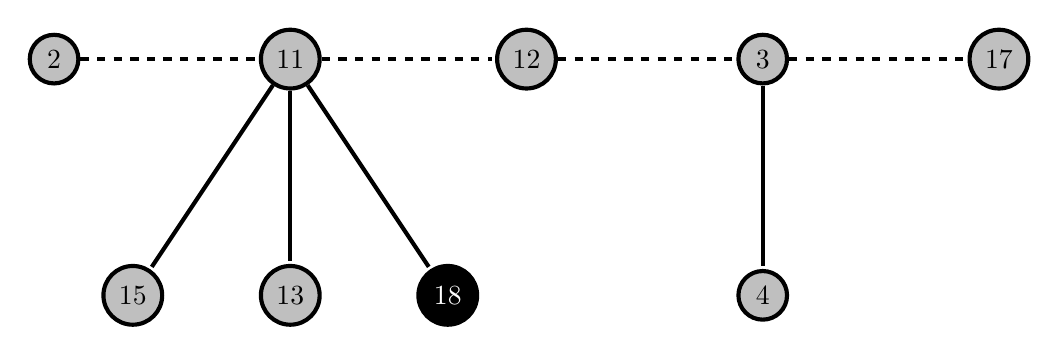
\begin{tikzpicture}[-,>=stealth,shorten >=1pt,auto,
      main node/.style={circle,draw}, line width=1.5pt]
  \node[main node,fill=lightgray] (a) at (0,0) {2};
  \node[main node,fill=lightgray] (b) at (3,0) {11};
  \node[main node,fill=lightgray] (f) at (1,-3) {15};
  \node[main node,fill=lightgray] (g) at (3,-3) {13};
  \node[main node,fill=black,text=white] (h) at (5,-3) {18};
  \node[main node,fill=lightgray] (c) at (6,0) {12};
  \node[main node,fill=lightgray] (d) at (9,0) {3};
  \node[main node,fill=lightgray] (i) at (9,-3) {4};
  \node[main node,fill=lightgray] (e) at (12,0) {17};
  \path[every node/.style={font=\small}]
  (a) edge[dashed] (b)
  (b) edge[dashed] (c)
  (c) edge[dashed] (d)
  (d) edge[dashed] (e)
  (b) edge (f)
  (b) edge (g)
  (b) edge (h)
  (d) edge (i)
  ;
  \end{tikzpicture}
  \end{center}

Hvilke af nedenstående operationer på $H$ får værdien af potentialfunktionen til at \emph{stige}?
(Bemærk at CLRS ikke indeholder pseudokode for {\sc Fib-Heap-Minimum}, men kun en skriftlig beskrivelse.)
\fleresvar
\mulighederstart
\svar {\sc Fib-Heap-Minimum}($H$)
\svar {\sc Fib-Heap-Insert}($H$, 1) \korrekt
\svar {\sc Fib-Heap-Insert}($H$, 20) \korrekt
\svar {\sc Fib-Heap-Delete}($H$, 4)
\svar {\sc Fib-Heap-Delete}($H$, 18) 
\svar {\sc Fib-Heap-Decrease-Key}($H$, 11, 7)
\mulighederslut

\forklaring{
{\sc Fib-Heap-Minimum}(H) ændrer ikke datastrukturen og derfor heller ikke potentialfunktionen.
{\sc Fib-Heap-Insert} operationerne øger rodlistens længde $t(H)$ med 1, og dermed også $\Phi(H)$.
  {\sc Fib-Heap-Delete} operationer \emph{kan} resultere i nye markerede knuder men i dette tilfælde laves ingen markeringer fordi kun knuder i rodlisten mister et barn.
  {\sc Fib-Heap-Decrease-Key} operationen resulterer ikke i nogen {\sc Cut} operation, så potentialfunktionen ændres ikke.

}



\spoergsmaal{Stavudskæring}
Betragt algoritmen {\sc Bottom-Up-Cut-Rod} beskrevet i CLRS sektion 14.1.
Hvilket array~$r$ returnerer algoritmen på input $p = \langle 2, 3, 5, 7, 11, 12 \rangle$, med $n=6$?
\etsvar
\mulighederstart
\svar $r = \langle0,2,4,6,8,10,12\rangle$
\svar $r = \langle0,2,4,6,8,11,12\rangle$
\svar $r = \langle0,2,4,6,8,11,13\rangle$ \korrekt
\svar $r = \langle0,2,4,6,9,12,13\rangle$
\svar $r = \langle0,2,4,6,9,12,14\rangle$
\svar $r = \langle0,2,4,6,9,13,14\rangle$
\mulighederslut

\forklaring{
Inden første iteration har vi $r[0] = 0$.
Efter 1 iteration har vi $r[1] = 2$ (maksimum fås ved at tage 1 stav af længde 1).
Efter 2 iterationer har vi $r[2] = 4$ (maksimum fås ved at tage 2 stave af længde 1).
Efter 3 iterationer har vi $r[3] = 6$ (maksimum fås ved at tage 3 stave af længde 1).
Efter 4 iterationer har vi $r[4] = 8$ (maksimum fås ved at tage 4 stave af længde 1).
Efter 5 iterationer har vi $r[5] = 11$ (maksimum fås ved at tage en stav af længde 5, andre løsninger giver en værdi på højst~10).
Efter 6 iterationer har vi $r[6] = 13$ (maksimum fås ved at tage en stav af længde 5 og en af længde 1, andre løsninger giver en værdi på højst 12).
}


\spoergsmaal{Huffman koder}
Vi betragter algoritmen til konstruktion af Huffman koder i CLRS sektion 15.3 kørt på alfabetet $C =\{a, b, c, d, e\}$ med frekvenser $f_a=50$, $f_b=42$, $f_c=11$, $f_d=22$, $f_e=33$.
Hvor langt er det \emph{korteste} kodeord (eng.~\emph{codeword}) i den beregnede Huffman kode?
\etsvar
\mulighederstart
\svar Længde 1
\svar Længde 2 \korrekt
\svar Længde 3
\svar Længde 4
\mulighederslut

\forklaring{Algoritmen beregner dette træ (tegnet uden 0-1 labels på kanterne), der indeholder tre kodeord (for a,b,e) af længde 2 men ingen kodeord af længde 1:\medskip
\begin{center}
    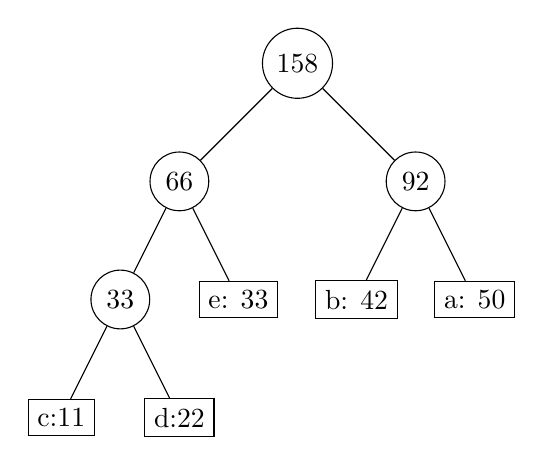
\begin{tikzpicture}[level distance=1.5cm,  level 1/.style={sibling distance=3cm},  level 2/.style={sibling distance=1.5cm}]
        \node [circle, draw] {158}
          child {node [circle, draw] {66}
            child {node [circle, draw] {33}
              child {node [rectangle, draw] {c:11}}
              child {node [rectangle, draw] {d:22}}
            }
            child {node [rectangle, draw] {e: 33}}
          }
          child {node [circle, draw] {92}
            child {node [rectangle, draw] {b: 42}}
            child {node [rectangle, draw] {a: 50}}
          };
      \end{tikzpicture}
\end{center}


}



\spoergsmaal{Rød-sorte søgetræer I}
Betragt et rød-sort binært søgetræ $T$ (eng.~\emph{red-black binary search tree}), som beskrevet i CLRS kapitel 13.
Betragt nedenstående træ, hvor alle blade er udeladt (som på CLRS figur 13.1.c) og én indre knude er uspecificeret:

\begin{center}
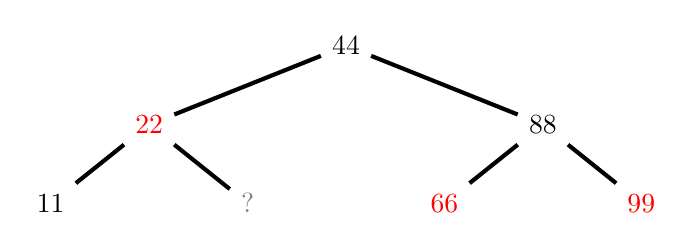
\begin{tikzpicture}[-,>=stealth,level/.style={sibling distance = 5cm/#1,
    level distance = 1cm}, line width=1.5pt] 
  \node [black] {44}
      child{ node [red] {22} 
              child{ node [black] {11}
              }
              child{ node [gray] {?}
              }                            
      }
      child{ node [black] {88}
            child{ node [red] {66}}
            child{ node [red] {99}}
          }
  ; 
  \end{tikzpicture}  
\end{center}

\medskip

Hvilke knuder er mulige på positionen markeret med ?, hvis træet skal overholde invarianterne for et rød-sort binært søgetræ?
\etsvar
\mulighederstart
\svar Sorte knuder med værdi mindst 11 og højst 22
\svar Sorte knuder med værdi mindst 22 og højst 44 \korrekt
\svar Sorte knuder med værdi mindst 11 og højst 66
\svar Røde knuder med værdi mindst 11 og højst 22
\svar Røde knuder med værdi mindst 22 og højst 44
\svar Røde knuder med værdi mindst 11 og højst 66
\mulighederslut
\forklaring{ Knuden skal være sort fordi dens forælder er rød, ellers ville en rød-sort invariant være overtrådt.
Værdien skal være mellem 22 og 44 fordi træet er et søgetræ.
}




\spoergsmaal{Rød-sorte søgetræer II}
Betragt et rød-sort binært søgetræ $T$ (eng.~\emph{red-black binary search tree}), som beskrevet i CLRS kapitel 13.
Hvilke udsagn gælder for et hvilket som helst rød-sort binært søgetræ?
\fleresvar
\mulighederstart
\svar Højden og den sorte højde er altid den samme for et blad (en ekstern knude). \korrekt
\svar Den sorte højde stiger med 1 når man går ét skridt op i træet.
\svar Antal røde knuder er altid mindre end antal sorte knuder (inkl.~blade).  \korrekt
\svar Roden er altid sort. \korrekt
\svar Der kan være både røde og sorte blade (eksterne knuder).
\svar Når en knude indsættes er den rød, og den forbliver rød indtil en senere indsætning eller sletning.
\svar Når en knude slettes, er det altid nødvendigt at omfarve og/eller rotere.
\mulighederslut

\forklaring{
  1. Eksterne knuder har ingen børn og deres højde er derfor 0. Den sorte højde af en knude X er antallet af sorte knuder på en vilkårlig simpel sti fra X (X ikke medregnet) ned til et blad; ifølge de rød-sorte egenskaber er dette antal det samme for alle sådanne stier. Hvis X er en ekstern knude, er dens sorte højde derfor lig med 0.
  2. Den sorte højde af en rød knude er lig med den sorte højde af dens far.
  3. Begge børn af en rød knude er altid sorte, og da hver knude højst har én far, er der mindst dobbelt så mange sorte knuder som røde. Da der altid er mindst én sort knude (fx roden eller et blad), er antallet af røde knuder altid mindre end antallet af sorte knuder.
  4. Per definition af et rød-sort BST.
  5. Ifølge definitionen af rød-sorte knuder er eksterne knuder altid sorte.
  6. Simpelt modeksempel: Når en knude indsættes i et tomt rød-sort træ, får den rød farve. Dens farve ændres til sort fordi den er rod.
  7. Simpelt modeksempel: Hvis den knude der slettes er rød og begge dens børn er blade (fx en rød knude hvis far er en sort rod), fjernes den blot, uden omfarvning eller rotation, fordi ingen af de rød-sorte egenskaber brydes. I CLRS's {\sc RB-Delete} kaldes {\sc RB-Delete-Fixup} kun når den fjernede eller flyttede knude er sort.
}



\spoergsmaal{Mindste udspændende træ}
Betragt mindste udspændende træ (eng.~\emph{minimum spanning tree}) problemet på denne graf:
\begin{center}
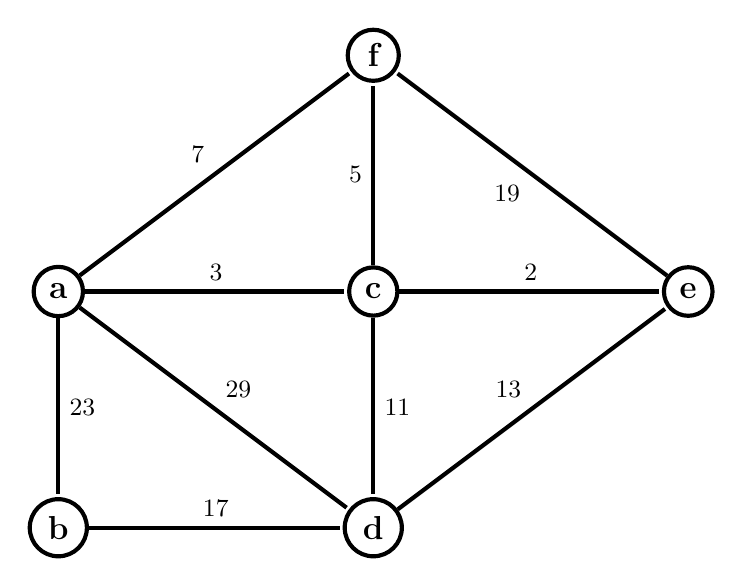
\begin{tikzpicture}[-,>=stealth,shorten >=1pt,auto,
  main node/.style={circle,draw,font=\large\bfseries}, line width=1.5pt]
\node[main node] (a) at (2,1.5) {a};
\node[main node] (b) at (2,-1.5) {b};
\node[main node] (c) at (6,1.5) {c};
\node[main node] (d) at (6,-1.5) {d};
\node[main node] (e) at (10,1.5) {e};
\node[main node] (f) at (6,4.5) {f};

\path[every node/.style={font=\small}]
(a) edge node {23} (b) 
edge node {3} (c)
edge node {29} (d) 
edge node {7} (f)
(b) edge node {17} (d)
(c) edge node {11} (d) 
edge node {2} (e) 
edge node {5} (f) 
(d) edge node {13} (e)
(e) edge node {19} (f); 
\end{tikzpicture}
\end{center}
Hvilke kanter er med i det mindste udspændende træ (som er unikt)?
\fleresvar
\mulighederstart
\svar \{a,b\} 
\svar \{a,c\} \korrekt
\svar \{a,d\} 
\svar \{a,f\} 
\svar \{b,d\} \korrekt
\svar \{c,d\} \korrekt
\svar \{c,e\} \korrekt
\svar \{c,f\} \korrekt
\svar \{d,e\} 
\svar \{e,f\}
\mulighederslut
\forklaring{Mindste udspændende træ kan findes ved at køre fx Kruskal's eller Prim's algoritme. Kruskal's algoritme tilføjer kanterne i vægtrækkefølge, dvs.~starter med \{c,e\}, \{a,c\}, \{c,f\}, springer over \{a,f\} fordi det ville skabe en kreds, og tilføjer \{c,d\}, springer over \{d,e\} fordi det ville skabe en kreds, og afslutter med \{b,d\}. }



\spoergsmaal{Snit og sikre kanter} 
Betragt følgende uorienterede, vægtede graf med knudemængde $V=\{a,b,c,d,e,f\}$:\\
\begin{center}
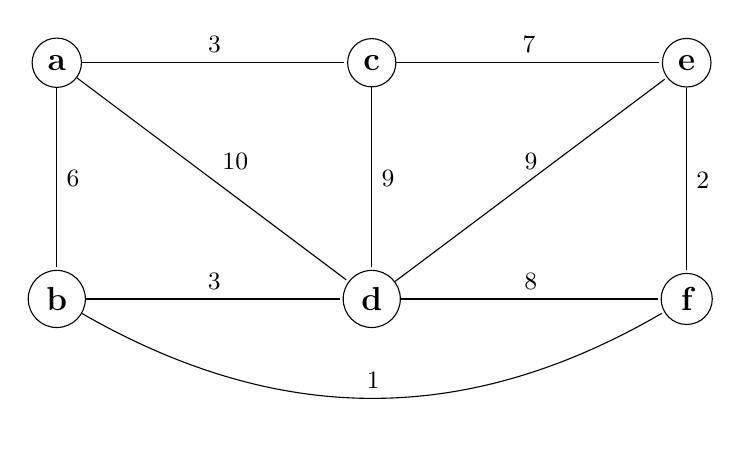
\begin{tikzpicture}[-,>=stealth,shorten >=1pt,auto,
    main node/.style={circle,draw,font=\large\bfseries}]
\node[main node] (a) at (2,1.5) {a};
\node[main node] (b) at (2,-1.5) {b};
\node[main node] (c) at (6,1.5) {c};
\node[main node] (d) at (6,-1.5) {d};
\node[main node] (e) at (10,1.5) {e};
\node[main node] (f) at (10,-1.5) {f};

\path[every node/.style={font=\small}]
(a) edge node {6} (b)
edge node {3} (c)
edge node {10} (d)
(b) edge node {3} (d)
edge[bend right=30] node {1} (f)
(c) edge node {9} (d)
edge node {7} (e)
(d) edge node {8} (f)
(e) edge node {2} (f)
(d) edge node[above] {9} (e);
\end{tikzpicture}
\end{center}
%
Hvilke kanter er lette kanter for snittet $(S,V-S)$ (eng.~\emph{light edges for the cut $(S,V-S)$}), hvor $S=\{a,b,e,f\}$?
\fleresvar
\mulighederstart
\svar \{a,b\}
\svar \{a,c\} \korrekt
\svar \{a,d\}
\svar \{b,d\} \korrekt
\svar \{b,f\}
\svar \{c,d\}
\svar \{c,e\}
\svar \{d,e\}
\svar \{d,f\}
\svar \{e,f\}
\mulighederslut
\forklaring{Den mindste vægt for kanter i snittet er 3, og de to snitkanter \{a,c\} og \{b,d\} har denne vægt.
Kanterne \{b,f\} og \{e,f\} har lavere vægte men er ikke snitkanter.
}



\spoergsmaal{Valg af algoritme}
Betragt følgende orienterede, vægtede graf:
\begin{center}
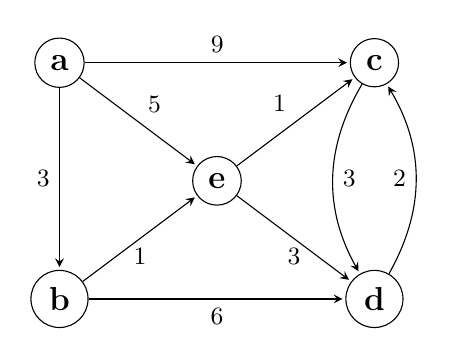
\begin{tikzpicture}[->,>=stealth,shorten >=1pt,auto,
    main node/.style={circle,draw,font=\large\bfseries}]
\node[main node] (a) at (2,1.5) {a};
\node[main node] (b) at (2,-1.5) {b};
\node[main node] (c) at (6,1.5) {c};
\node[main node] (d) at (6,-1.5) {d};
\node[main node] (e) at (4,0) {e};
\path[every node/.style={font=\small}]
(a) edge node[left] {3} (b)
edge node[above] {9} (c)
edge node {5} (e)
(b) edge node[below] {6} (d)
edge node[below] {1} (e)
(c) edge[bend right] node {3} (d)
(d) edge[bend right] node {2} (c)
(e) edge node {1} (c)
edge node[below] {3} (d);
\end{tikzpicture}
\end{center}

\medskip\noindent
Hvilken af nedenstående algoritmer fra CLRS er det bedste valg til at beregne en korteste vej (eng.~\emph{single-source shortest-path}) fra startknude {\bf a} til slutknude {\bf d}? Der lægges vægt på korrekthed og god asymptotisk køretid for den valgte algoritme. Du kan antage at kantvægtene, i lighed med ovenstående graf, ligger mellem 1 og 9.
\etsvar
\mulighederstart
\svar Bellman-Ford algoritmen
\svar Bredde-først søgning
\svar Dijkstra's algoritme \korrekt
\svar Kruskal's algoritme
\svar Prim's algoritme
\mulighederslut
\forklaring{Bellman-Ford algoritmen og Dijkstra's algoritme beregner begge en korteste vej, men da grafen ikke har negative vægte er Dijkstra et bedre valg fordi den er asymptotisk hurtigere.}



\spoergsmaal{Korteste veje}
Betragt korteste veje problemet (eng.~\emph{single-source shortest-paths problem}) med startknude {\bf a} på følgende graf:
\begin{center}
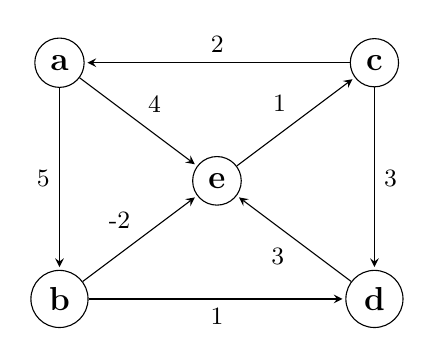
\begin{tikzpicture}[->,>=stealth,shorten >=1pt,auto,
    main node/.style={circle,draw,font=\large\bfseries}]
\node[main node] (a) at (2,1.5) {a};
\node[main node] (b) at (2,-1.5) {b};
\node[main node] (c) at (6,1.5) {c};
\node[main node] (d) at (6,-1.5) {d};
\node[main node] (e) at (4,0) {e};
\path[every node/.style={font=\small}]
(a) edge node[left] {5} (b)
edge node {4} (e)
(b) edge node[below] {1} (d)
edge node {-2} (e)
(c) edge node {3} (d)
edge node[above] {2} (a)
(d) edge node {3} (e)
(e) edge node {1} (c);
\end{tikzpicture}
\end{center}

\medskip\noindent
Hvilke kanter er med i korteste-vej træet (eng.~\emph{shortest-path tree}) med startknude {\bf a}?
\fleresvar
\mulighederstart
\svar (a,b) \korrekt
\svar (a,e) 
\svar (b,d) \korrekt
\svar (b,e) \korrekt
\svar (c,a)
\svar (c,d) 
\svar (d,e) 
\svar (e,c) \korrekt 
\mulighederslut
\forklaring{Da der er negative vægte kan kanterne i træet findes ved at køre Bellman-Ford algoritmen, der giver det angivne output (som i dette tilfælde er unikt).}




\spoergsmaal{Beregningsgeometri}
Det konvekse hylster (eng.~\emph{convex hull}) af en punktmængde kan beregnes med algoritmer fra CLRS digitalt kapitel 33.
Betragt nedenstående punktmængde $P$:
\begin{center}
\begin{tikzpicture}[scale=0.5]

% Manually define coordinates for points
\coordinate (p1) at (2, 3);
\coordinate (p2) at (5, 7);
\coordinate (p3) at (8, 1);
\coordinate (p4) at (1, 6);
\coordinate (p5) at (4, 5);
\coordinate (p6) at (7, 2);
\coordinate (p7) at (3, 8);
\coordinate (p8) at (6, 4);
\coordinate (p9) at (9, 9);

% Draw and label points
\foreach \i in {1,2,...,9} {
    \fill (p\i) circle (2pt) node[above] {$p_\i$};
}
\end{tikzpicture}
\end{center}

\noindent
Hvilke udsagn er korrekte? (De to første relaterer til punktmængden $P$, de øvrige handler om generelle punktmængder.)
\fleresvar
\mulighederstart
\svar Det konvekse hylster for $P$ har $h=5$ hjørner. \korrekt
\svar Punktet $p_2$ er ikke et hjørne i det konvekse hylster for $P$. \korrekt
\svar Graham's scan er aldrig asymptotisk langsommere end Jarvis' march.
\svar Jarvis' march tager tid $\Theta(n^2)$ på et værste input med $n$ knuder. \korrekt
\svar Graham's scan tager tid $\Theta(n^2)$ på et værste input med $n$ knuder.
\mulighederslut
\forklaring{Det konvekse hylster har hjørnerne $p_4,p_7,p_9,p_3,p_1$, øvrige punkter er indeni det konvekse hylster. Graham's scan er langsommere end Jarvis' march når antal hjørner på det konvekse hylster er $h=o(\log n)$. Når $h=\Theta(n)$, fx hvis alle punkter ligger på en cirkel, tager Jarvis' march $\Theta(n^2)$ tid. Graham's scan tager $O(n \log n)$ tid.}


\multiplechoiceslut

\newpage


\section*{Skriftlige opgaver}\label{sec:written}

{\bf Skriftlige opgaver} afleveres som et Word dokument i ITX systemet.
Der er mulighed for at tegne og skrive på tablet, og indsætte i dokumentet.
\begin{itemize}
    \item Brug \emph{én side til hvert delspørgsmål, i samme rækkefølge som i opgavesættet.} 
    \item Delspørgsmålets nummer/bogstav (fx 19 eller 20.a) skal fremgå.
\end{itemize}



\section{Længste fælles delsekvens (5\%)}

Vi betragter algoritmen til længste fælles delsekvens (eng.~\emph{longest common subsequence}) i CLRS sektion 14.4.

\punkt{a)}{
Tegn det array $c$ som algoritmen udfylder på følgende input:
\begin{center}
$X = \langle N, E, O, N\rangle $ og $Y = \langle A, N, N, O, N, A\rangle$.
\end{center}
\medskip
\noindent
Tilføj pile ($\uparrow$, $\nwarrow$, $\leftarrow$), der forklarer tallene i $c$, som i CLRS Figur 14.8 og \emph{angiv den længste fælles delsekvens}.
}

\forklaring{For overskuelighedens skyld inkluderer vi de to strenge i kanten af $c$, ligesom i CLRS Figur 14.8.\medskip
\begin{center}
\begin{tabular}{c||c|c|c|c|c|c|c||}
    & & A & N & N & O & N & A \\
    \hline
    \hline
     & 0 & 0 & 0 & 0 & 0 & 0 & 0\\
     \hline
    N & 0 & $\uparrow$0 & $\nwarrow$1 & $\nwarrow$1 & $\leftarrow$1 & $\nwarrow$1 & $\leftarrow$1\\
    \hline
    E & 0 & $\uparrow$0 & $\uparrow$1 & $\uparrow$1 & $\uparrow$1 & $\uparrow$1 & $\uparrow$1\\
    \hline
    O & 0 & $\uparrow$0 & $\uparrow$1 & $\uparrow$1 & $\nwarrow$2 & $\leftarrow$2 & $\leftarrow$2\\
    \hline
    N & 0 & $\uparrow$0 & $\nwarrow$1 & $\nwarrow$2 & $\uparrow$2 & $\nwarrow$3 & $\leftarrow$3\\
    \hline
    \hline
\end{tabular}
\end{center}
(I nogle tilfælde er der et valg mellem $\uparrow$ og $\leftarrow$, det lægger vi ikke vægt på når der gives point.) Længste fælles delsekvens er NON.
}




\section{Induktionsbevis for køretid (8\%)}

En algoritme tager tid $T(n) = n^2 + \sum_{i=1}^n \binom{i+1}{2}$ på et input af størrelse $n$, hvor $\binom{i+1}{2} = \tfrac{i(i+1)}{2}$.
Vi ønsker at vise at køretiden overholder $T(n) \leq 2\, n^3$ for alle $n\geq 1$.

\punkt{a)}{ Vis at $T(1) = 2$.
}
\forklaring{$T(1) = 1^2 + \sum_{i=1}^1 \binom{i+1}{2} = 2$.}

\punkt{b)}{ Vis $T(n) \leq 2 n^3$ ved induktion.
}
\forklaring{
Fra del a) ved vi at $T(n) \leq 2\, n^3$ gælder i basistilfældet $n=1$.
I induktionsskridtet antager vi at $T(n-1) \leq 2\, (n-1)^3$ (induktionshypotese).
Vi har at 
\begin{align*}
T(n) & = n^2 + \sum_{i=1}^n \tbinom{i+1}{2}\\
& = T(n-1) + (2n-1) + \tbinom{n+1}{2}\\
& \leq 2 (n-1)^3 + (2n - 1) + \tfrac{n(n+1)}{2}\\
& = (2\, n^3 - 6n^2 + 6n - 2) + (2n - 1) + (n^2 / 2 + n/2)\\
& = 2\, n^3 - 5.5 n^2 + 8.5n - 2.5\\
& < 2\, n^3 \enspace .
\end{align*}
Den første ulighed bruger induktionshypotesen, den anden bruger at $- 5.5 n^2 + 8.5n - 2.5$ er negativt for $n\geq 2$.
Dette færdiggør induktionsskridtet.
}



\section{Køretid (9\%)}

Antag i det følgende at $A[1: n]$ er et array af $n$ heltal og at $k$ er et heltal.
Vi betragter disse to funktioner:
\begin{codebox}
    \Procname{$\proc{PrefixSum}(A, n, k)$}
    \li $s = 0$
    \li \If $k > n$ \Do 
    \li $t = n$ \End
    \li \Else \Do
    \li $t=k$ \End
    \li \For $i = 1$ \To $t$ \Do
    \li $s = s + A[i]$ \End
    \li \Return $s$
\end{codebox}
\begin{codebox}
  \Procname{$\proc{PowerSums}(A, n)$}
  \li $k = 1$
  \li $s = 0$
  \li \While $k < n$ \Do
  \li $s = s + \proc{PrefixSum}(A, n, k)$ 
  \li $k = 2\cdot k$ \End
  \li \Return $s$
\end{codebox}


\punkt{a)}{ Angiv en asymptotisk grænse på køretiden for {\sc PrefixSum} med brug af store-$\Theta$ notation, som funktion af variablerne $n$ og $k$. Argumentér kort for dit svar.}

\forklaring{
Køretiden er $\Theta(\min(n,k))$ fordi {\bf for}-løkken laver $t$ iterationer, hver iteration tager konstant tid, og {\bf if} sætningen i linje 2-5 sikrer at $t=\min(n,k)$.}

\punkt{b)}{ Angiv antal iterationer for {\bf while} løkken i {\sc PowerSums}  med brug af store-$\Theta$ notation, som funktion af $n$. Argumentér kort for dit svar.}

\forklaring{
Løkken starter med $k=1$, fordobler værdien af $k$ i hver iteration, og terminerer når $k \geq n$.
Per definition af totalslogaritmen af $n\geq 1$ er antal iterationer præcis $\lceil \lg n\rceil$.
Dvs.~antal iterationer er $\Theta(\lg n)$.
}

\punkt{c)}{ Angiv en øvre grænse for køretiden af {\sc PowerSums} og udtryk den i store-$\Theta$ notation, som en simpel funktion af $n$. Argumentér kort for dit svar.}

\forklaring{
Ifølge spørgsmål a), og fordi $k<n$, er omkostningen ved hvert kald $\Theta(k)$.
I iteration $i=0,1,\dots,\lceil \lg n\rceil-1$ er $k=2^i$, så med brug af del b) bliver den samlede omkostning  $\Theta(\sum_{i=0}^{\lceil \lg n\rceil-1} 2^i)$, som er $\Theta(n)$ da summen er en geometrisk række der domineres af det største led $2^{\lceil \lg n\rceil-1} < n$.
Denne analyse er præcis da det sidste kald af {\sc PrefixSum} har $k \geq n/2$, og dette kald alene tager tid $\Omega(n)$.
}






\section{Minimax udspændende træ (6\%)}\label{sec:last}
Betragt en vægtet, ikke-orienteret og sammenhængende graf $G=(V,E)$. Et udspændende træ i $G$ hvor vægten af den tungeste kant er mindst muligt kaldes et \emph{MiniMax Udspændende Træ} (MMUT).

\medskip
\noindent
{\bf Eksempel:} I denne graf udgør de markerede kanter et MMUT. Den maksimale vægt i træet er 4, og der findes ikke noget udspændende træ med en mindre maksimal vægt.

\begin{center}
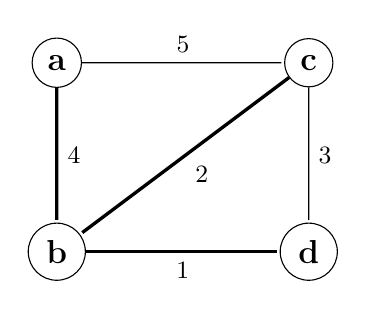
\begin{tikzpicture}[-,scale=0.8,>=stealth,shorten >=1pt,auto,
  main node/.style={circle,draw,font=\large\bfseries}]
\node[main node] (a) at (2,1.5) {a};
\node[main node] (b) at (2,-1.5) {b};
\node[main node] (c) at (6,1.5) {c};
\node[main node] (d) at (6,-1.5) {d};

\path[every node/.style={font=\small}]
(a) edge[very thick] node {4} (b)
edge node {5} (c)
(b) edge[very thick] node[below] {1} (d)
(c) edge node {3} (d)
edge[very thick] node {2} (b);
\end{tikzpicture}
\end{center}


\punkt{a)}{ Giv et eksempel på at et MMUT ikke altid er et mindste udspændende træ.}

\forklaring{ I denne graf findes et MMUT med maksimal vægt 2 og total vægt 4. Et mindste udspændende træ har vægt 3.
  \begin{center}
    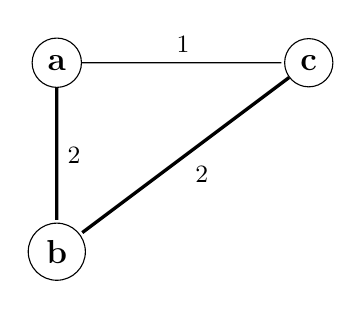
\begin{tikzpicture}[scale=0.8,-,>=stealth,shorten >=1pt,auto,
      main node/.style={circle,draw,font=\large\bfseries}]
    \node[main node] (a) at (2,1.5) {a};
    \node[main node] (b) at (2,-1.5) {b};
    \node[main node] (c) at (6,1.5) {c};
    
    \path[every node/.style={font=\small}]
    (a) edge[very thick] node {2} (b)
    edge node {1} (c)
    (c) edge[very thick] node {2} (b);
    \end{tikzpicture}
    \end{center}
}

\punkt{b)}{ Bevis at et mindste udspændende træ altid er et MMUT. }

\forklaring{Bevis ved modstrid. 
Lad $T$ betegne et mindste udspændende træ (MUT) og antag at det ikke er et MMUT. 
Lad $T'$ betegne et MMUT. 
Lad $e$ betegne kanten med den største vægt i $T$ og lad $e'$ betegne kanten med den største vægt i $T'$. Da $T$ ikke er et MMUT så må da gælde at $|e| > |e'|$ og $e$ er ikke i $T'$. 
Når $e$ tilføjes til $T'$, dannes der en kreds. 
I denne kreds findes en kant der krydser snittet defineret ved sammenhængskomponenterne der opstår hvis $e$ fjernes fra $T$, dvs.~at $e$ er ikke minimal i snittet, i modstrid med antagelsen.
%Alle kanter i denne kreds har mindre vægt end $e$. 
%Det betyder at alle snit med $e$ som krydsende kant indeholder en kant med mindre vægt end vægten af $e$. 
%Med andre ord er $e$ ikke en sikker kant i noget snit. 
%Men så kan $e$ ikke være med i noget MUT. 
%Det er i modstrid med at $e$ er i $T$.
}


\label{page:last}
